\chapter{Eliminación de palabras}


Los capítulos anteriores se han enfocado en tratar a las migraciones de palabras como consecuencias de eventos donde  las lenguas están involucradas. La clasificación de los $n$-gramas en palabras funcionales y palabras de contenido, y la posterior eliminación de las palabras funcionales, facilitó encontrar las relaciones con los eventos y establecer una cuantificación para la influencia entre idiomas (llamada uso), pero ¿qué sucedería con esta cantidad si se realizaran otras reglas para eliminar ciertas palabras?

Esta pregunta ha llevado a la construcción de un nuevo algoritmo que limite a las palabras,  reduciendo el conjunto de las migraciones y obteniendo nuevos valores para el uso entre idiomas.  Elegidos una pareja de idioma origen \textit{A} e idioma receptor \textit{B}, el proceso es el siguiente. 


\begin{enumerate}
	
	\item Se toma la lista de los préstamos acumulados de \textit{A} en \textit{B},  este conjunto se denotará como \textbf{conjunto original}.
	
	\item Se escogen de forma aleatoria un conjunto de letras (desde una hasta diez), y se descartan de los préstamos acumulados a todas las palabras cuya primer letra sea alguna de las elegidas; siendo este nuevo grupo el \textbf{conjunto reducido}.
	
	\item Se establece un tercer grupo designado como \textbf{conjunto residuo}, conformado por todas las palabras eliminadas del conjunto original.  La unión del reducido y el residuo es el original. 
	
	\item En los tres conjuntos se emplea la ecuación \ref{ec.fuso}, para encontrar el uso de \textit{A} en \textit{B}. 	
	
\end{enumerate}

La intención de estas alteraciones no es desaparecer el conjunto de las migraciones, sino el reducirlas,   comparando el uso entre el conjunto original y el reducido.  Para poder decir que tanto ha cambiado el uso en los dos conjuntos, se utilizará el coeficiente de determinación $R^{2}$. 

El primer criterio importante sera al tomar el uso en el conjunto original como verdadero (ya que con el se establecieron los resultados del capítulo anterior) identificando sus valores para un tiempo $t$ como $O_{t}$, si el uso en el conjunto reducido para el mismo tiempo se denotan como  $v_{t}$ y el promedio de ellos es $\bar{v}$, entonces   el coeficiente de determinación queda definido como:

\begin{equation}
\label{ec.dif_uso}
R^{2} = 1 - \sum_{t} \frac{ \left( v_{t}- O_{t} \right)^{2}  }{ \left( v_{t} - \bar{v} \right)^{2} }
\end{equation}

Se define el concepto \textbf{conservación del uso} para aquellos pares de conjuntos donde el uso no cambie a pesar de las omisiones; la conservación es favorable si $R^{2}$ es próximo a 1.  Si la conservación no es favorable, es indicio de que para las migraciones, las palabras eliminadas son las más relevantes.

\section{Características de las eliminaciones}

El procedimiento de eliminar palabras, obteniendo el uso en los dos conjuntos y el coeficiente de determinación, se realizó dos mil veces por cada pareja de idiomas.  Tras las repeticiones, se distinguieron las siguientes características al graficar el uso del conjunto original y del reducido. 


\begin{itemize}
	
	\item Valores iguales. Punto a punto el conjunto reducido empalma al original, siendo las gráficas indistinguibles. La conservación del uso se da en todo el intervalo de tiempo. 
	
	\item Diferencia de alturas. Ambas gráficas muestran el mismo comportamiento, sin embargo existe una diferencia casi constante entre el uso original y el reducido. En este caso se dirá que el uso también se conserva ya que ambas graficas son las mismas, sólo que sus valores están desfasados. 
	
	\item Alteraciones por periodos.  Presenta periodos donde el uso de ambos conjuntos son completamente diferentes. La conservación se da por periodos de tiempo e incluso puede ser inexistente.
	
\end{itemize}

Para ilustrar las caracterizaras mencionadas, se exponen algunas graficas obtenidas, representado con un trazo continuo al uso del conjunto original, mientras que el uso en el conjunto reducido  es una serie de puntos.   Ya que los valores en el conjunto residuo son muy pequeños, se opto por no graficarlos, para no saturar la información. 

En cada grafica se especifica que idiomas se están tratando así como el conjunto de letras con las cuales se hicieron las eliminaciones. 

\clearpage

\begin{figure}[h!]
	\centering
	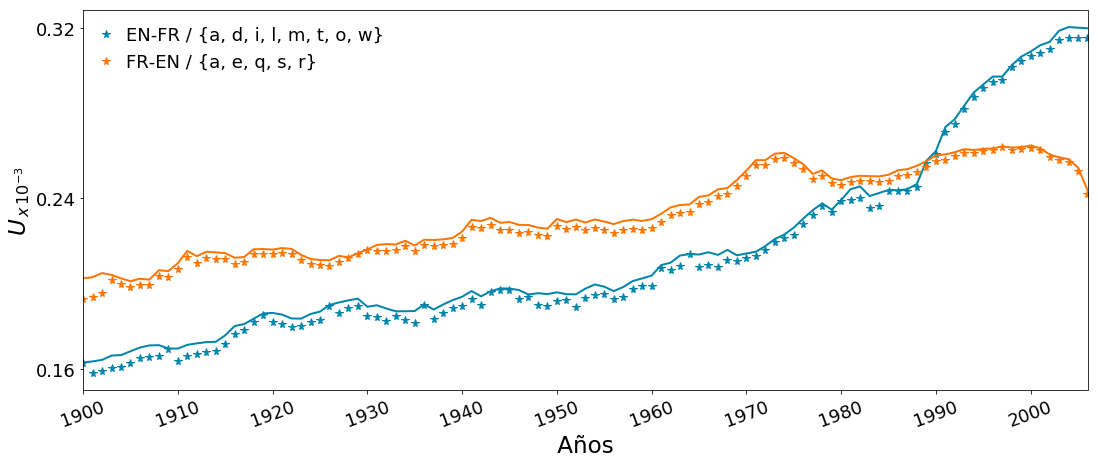
\includegraphics[scale=.38]{OM1.png}
	\label{fig.OM1}
	\caption{En ambas parejas de idiomas hay conservación del uso durante todo el siglo XX, al presentar valores iguales y  diferencia de alturas.}
\end{figure}


\begin{figure}[h!]
	\centering
	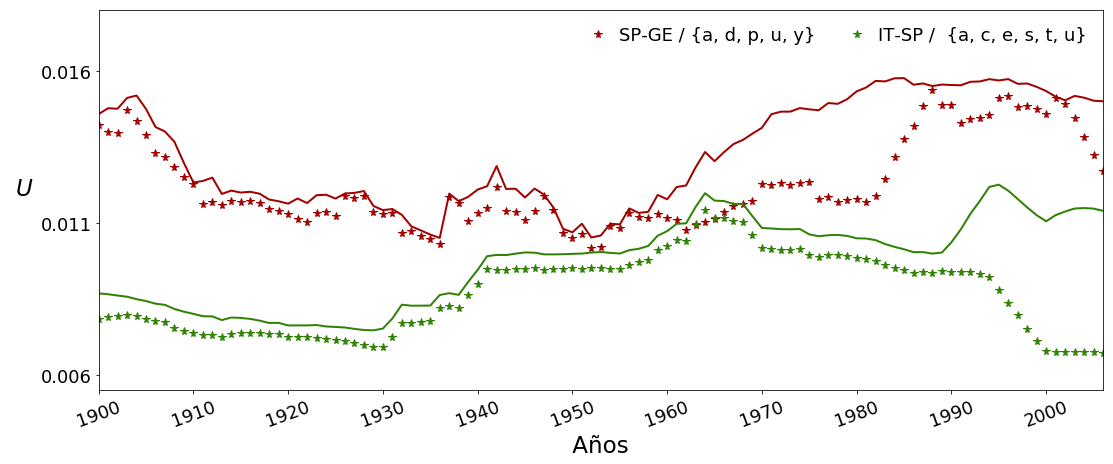
\includegraphics[scale=.38]{OM2.png}
	\label{fig.OM2}
	\caption{Sin conservación para el español-alemán entre 1960 y 1990,  debido a una alteración por periodos. Para el italiano-español el uso se conservo hasta mitad de siglo al existir una diferencia de alturas, en los últimos años se caracteriza por una alteración.}
\end{figure}

\clearpage
\begin{figure}[h!]
	\centering
	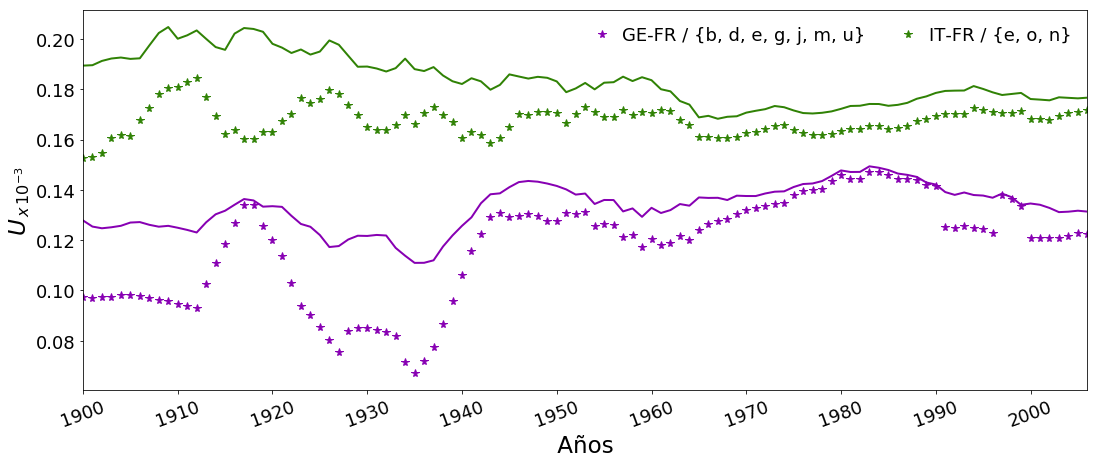
\includegraphics[scale=.38]{OM3.png}
	\label{fig.OM3}
	\caption{ En el italiano-francés se presenta conservación al  reducirse la diferencia de alturas conforme avanza el tiempo. El alemán-francés  presenta las tres características,  valores iguales  , alrededor de 1980  alteraciones entre 1920 y 1940, y deferencia de alturas  en los años restantes; la conservación dependerá del periodo  que se estudie.}
\end{figure}




La característica del uso y la conservación no siempre será la misma tras una eliminación con diferentes letras, sin embargo es posible decir de manera general si un idioma se conserva, para ello son útiles los resultados de las repeticiones. Si en cada idioma origen, se agrupan y promedian los valores del coeficiente de determinación,  se obtiene un valor promedio $\left \langle R^{2}  \right \rangle$ con el cual decir si el origen se conserva.  Los resultados de la tabla \ref{tab.conservacion} muestran el valor de  $\left \langle R^{2} \right \rangle$ de cada origen,  así como en cuales receptores la conservación fue mayor $R^{2}_{max}$ y  menor $R^{2}_{min}$.





\begin{table}[h!]
	\centering
	\begin{tabular}{cccc}
		\textbf{} & \textbf{$\left \langle R^{2} \right \rangle$} & \textbf{$R^{2}_{max}$} & \textbf{$R^{2}_{min}$} \\
		\textbf{inglés}   & 0.856 $\pm$ 0.147   &  IT 0.976 $\pm$ 0.001  & GE 0.778 $\pm$ 0.032  \\
		\textbf{francés}  & 0.839 $\pm$ 0.120   &  EN 0.951 $\pm$ 0.002  & GE 0.660 $\pm$ 0.020  \\
		\textbf{alemán}   & 0.753 $\pm$ 0.069   &  EN 0.805 $\pm$ 0.061  & SP 0.514 $\pm$ 0.332  \\
		\textbf{italiano} & 0.878 $\pm$ 0.147   &  FR 0.932 $\pm$ 0.008  & EN 0.687 $\pm$ 0.030  \\
		\textbf{español}  & 0.883 $\pm$ 0.053   &  IT 0.949 $\pm$ 0.006  & GE 0.818 $\pm$ 0.016                                                                
	\end{tabular}
	\caption{Los préstamos menos afectados por las eliminaciones son de origen español, siendo su conservación favorable en los receptores. El alemán es el que menos se conserva, afectado por ser el que menor cantidad de prestamos aporta a los demás idiomas.}
	\label{tab.conservacion}
\end{table}



\section{Comentarios del método}

El realizar diferentes elecciones para restringir a los préstamos, mostró que no importan cuales elementos conforman el corpus, la propiedad del uso es la misma. 

Individualmente los valores de uso de una única palabra pueden variar en los años de estudio y ser distintos a los de otra palabra, sin embargo al tratar a todo el conjunto, el uso se comporta de la misma  manera, sin importar los valores individuales de los elementos que lo conforman. 



